\documentclass{beamer}

\usetheme{egi}

\usepackage[utf8x]{inputenc}
\usepackage[T1]{fontenc}
\usepackage{cmap}
\usepackage{lmodern}
\usepackage[english]{babel}
\usepackage{listings}
\usepackage{color}
\usepackage{url}
\usepackage{hyperref}
\usepackage{fancyvrb,fancybox,calc}

% some helpful definitions
\definecolor{opennebulablue}{RGB}{0,145,197}
\definecolor{rubyred}{RGB}{204,52,45}

\newcommand{\opennebul}[1]{Open\textcolor{opennebulablue}{Nebul#1}}
\newcommand{\rocci}{\textcolor{rubyred}{r}\textcolor{opennebulablue}{OCCI}}

\newcommand\Fontsmaller{\fontsize{8}{9.2}\selectfont}
\newcommand\Fonttiny{\fontsize{7}{8.2}\selectfont}

\lstset{basicstyle=\footnotesize\ttfamily,
  numberstyle=\footnotesize\ttfamily,
  breaklines=true,
  breakatwhitespace=true,
  frame=single,
  numbers=left}


%
\title{cloud-init}
\subtitle{A webinar on contextualization}
\author{Enol Fern\'andez}
\date{2014-12-15, EGI Webinar}

%\AtBeginPart{\frame{\partpage}}

\begin{document}

\maketitle

\part{Overview}

%%%%%%%%%%%%%%%%%%%%%%%%%%%%%%%%%%%%%%%%%%%%%%%%%%%%%%%%%%%%%%%%%%%%%%%%%%%
\begin{frame}
  \frametitle{Agenda}
  \framesubtitle{}
  \begin{itemize}
    \item Brief introduction to FedCloud 
    \item Contextualization?
    \item Cloud-init 
    \begin{itemize}
        \item Basic usage 
        \item Cloud-config
        \item More use cases
    \end{itemize}
    \item Preparing your own images 
    \item Windows contextualization
    \item Q \& A
  \end{itemize}
\end{frame}

\part{FedCloud}

%%%%%%%%%%%%%%%%%%%%%%%%%%%%%%%%%%%%%%%%%%%%%%%%%%%%%%%%%%%%%%%%%%%%%%%%%%%
\begin{frame}
  \frametitle{EGI FedCloud}
  \framesubtitle{What is the EGI Federated Cloud}
    The EGI Federated Cloud is a federation of institutional private Clouds,
    offering Cloud Infrastructure as a Service to scientists in Europe
    and worldwide.

  \hfill\\

  \begin{columns}
    \column{0.7\textwidth}
        EGI Federated Cloud is based on:
        \begin{itemize}
            \item Standards and validation: federation is based on common
            Open-Standards – OCCI, CDMI, OVF, GLUE, etc...
            \item Heterogeneous implementation: no mandate on the cloud
            technology, the only condition is to expose the chosen
            interfaces and services.
        \end{itemize}

    \column{0.3\textwidth}
        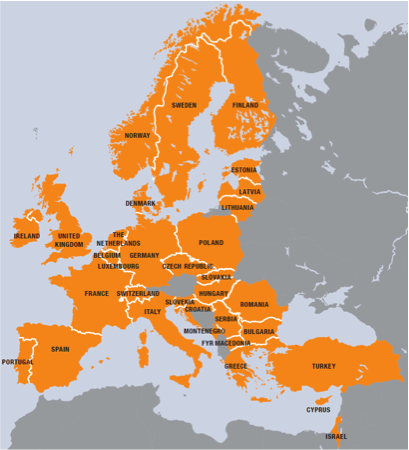
\includegraphics[width=\textwidth]{images/fedcloud_map}
  \end{columns}

  \hfill\\
      
\includegraphics[width=\textwidth]{images/fedcloud_usecases}
\end{frame}


%%%%%%%%%%%%%%%%%%%%%%%%%%%%%%%%%%%%%%%%%%%%%%%%%%%%%%%%%%%%%%%%%%%%%%%%%%%
\begin{frame}
  \frametitle{EGI FedCloud}
  \framesubtitle{Cloud Infrastructure Platform}

  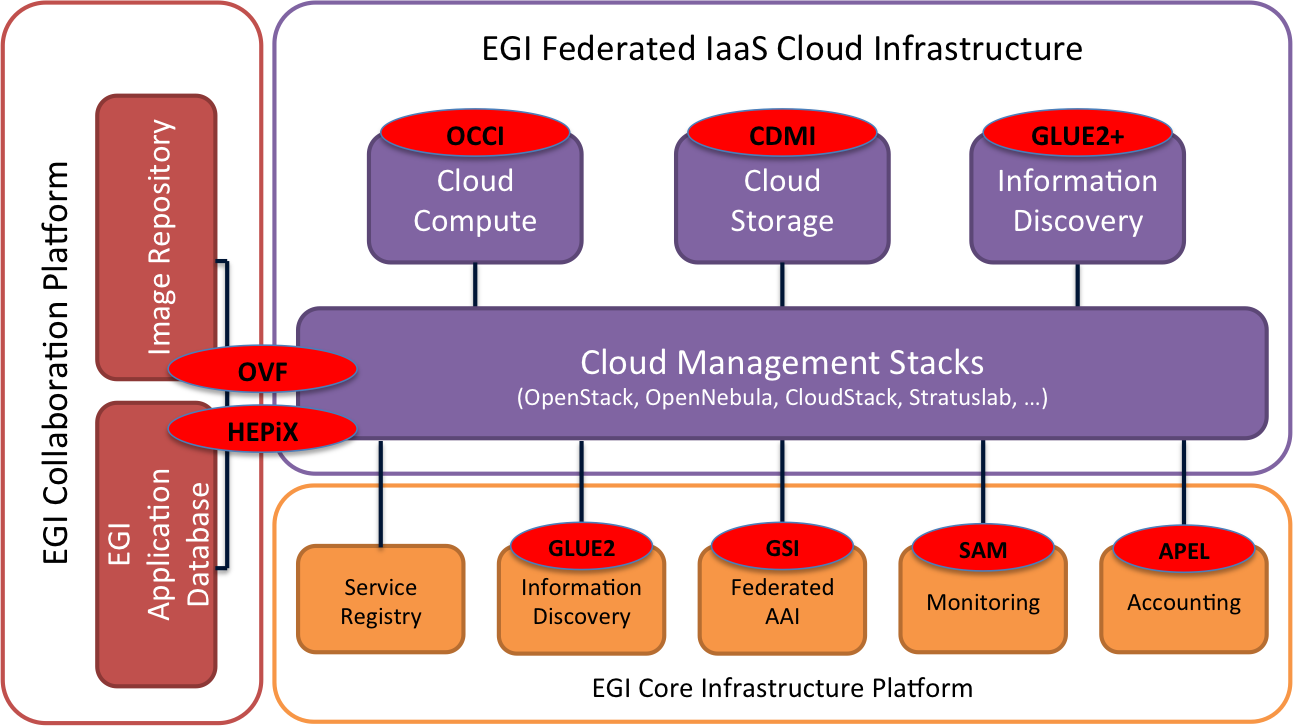
\includegraphics[width=\textwidth]{images/fedcloud_diagram}
\end{frame}

%%%%%%%%%%%%%%%%%%%%%%%%%%%%%%%%%%%%%%%%%%%%%%%%%%%%%%%%%%%%%%%%%%%%%%%%%%%
\begin{frame}
  \frametitle{EGI FedCloud}
  \framesubtitle{User workflows}

  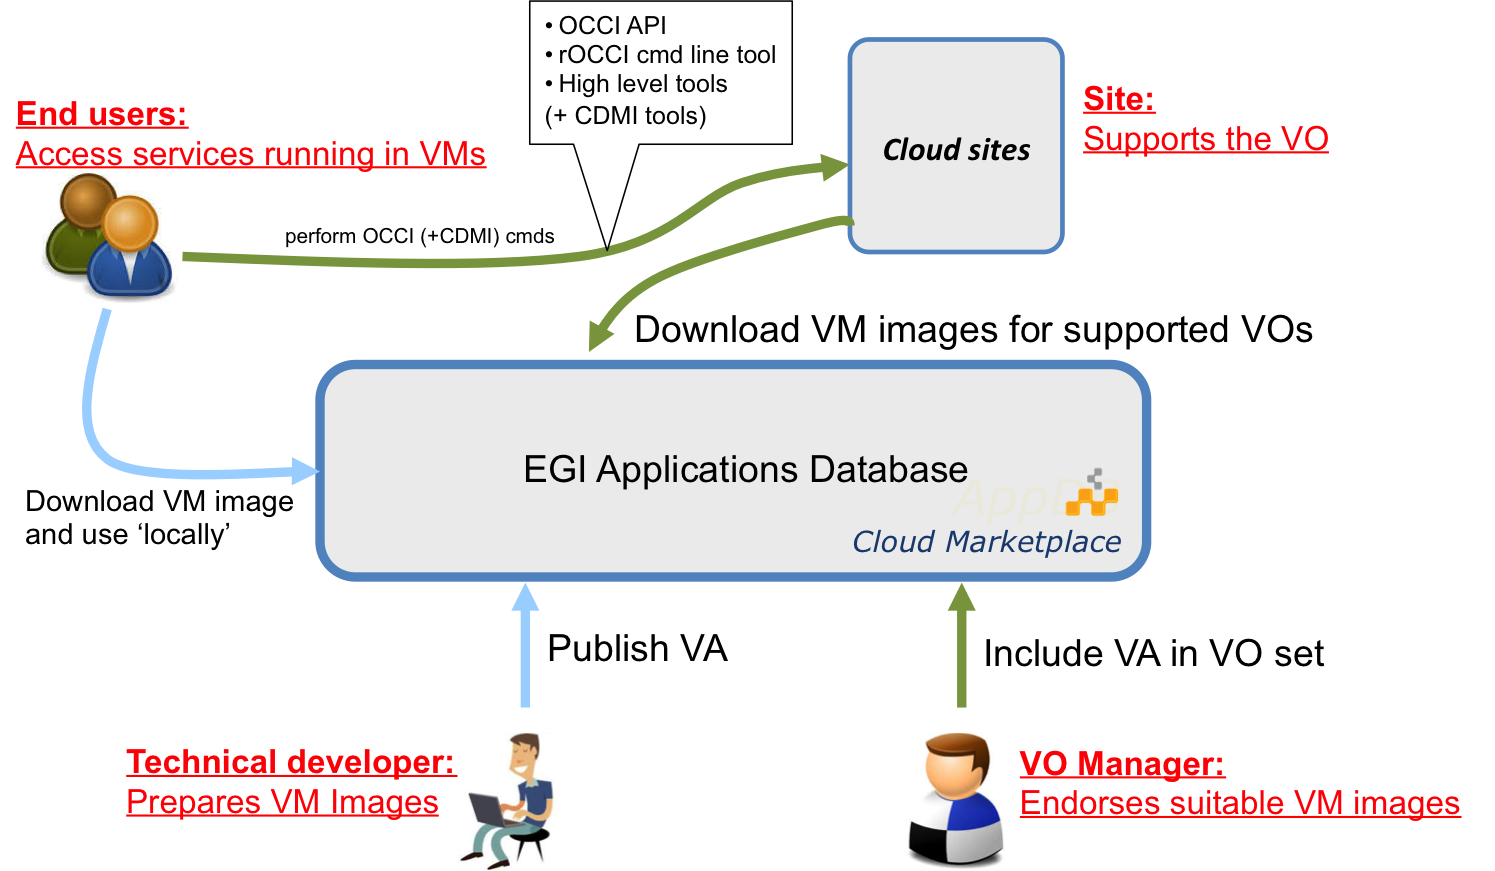
\includegraphics[width=\textwidth]{images/fedcloud_workflow}
\end{frame}

%%%%%%%%%%%%%%%%%%%%%%%%%%%%%%%%%%%%%%%%%%%%%%%%%%%%%%%%%%%%%%%%%%%%%%%%%%%


\part{ContextIntro}

%%%%%%%%%%%%%%%%%%%%%%%%%%%%%%%%%%%%%%%%%%%%%%%%%%%%%%%%%%%%%%%%%%%%%%%%%%%
\begin{frame}
  \frametitle{Contextualization}
  \framesubtitle{What -- Why?}

  \begin{block}{What?}
    Contextualization is the process of installing, configuring and
    preparing software upon boot time on a pre-defined virtual machine
    image (e.g. hostname, IP address, ssh keys, \dots)
  \end{block}

  \begin{block}{Why?}
    \begin{itemize}
      \item Configuration not known until instantiation (e.g. data location).
      \item Private Information (e.g. host certs)
      \item Software that changes frequently or under development.
      \item Not practical to create a new VM image for every possible configuration.
    \end{itemize}
  \end{block}
\end{frame}

%%%%%%%%%%%%%%%%%%%%%%%%%%%%%%%%%%%%%%%%%%%%%%%%%%%%%%%%%%%%%%%%%%%%%%%%%%%

\begin{frame}
  \frametitle{Contextualization}
  \framesubtitle{How?}

  \begin{block}{How?}
    \begin{itemize}
      \item Contextualization requires passing some data to the VMs on
            instantiation
      \item Standard OCCI API lacks such feature
      \item New mixins proposed and implemented in \rocci-server, OCCI-OS and Synnefo (i.e. all current RPs of EGI's Fedcloud!)
    \end{itemize}
  \end{block}

\end{frame}

%%%%%%%%%%%%%%%%%%%%%%%%%%%%%%%%%%%%%%%%%%%%%%%%%%%%%%%%%%%%%%%%%%%%%%%%%%%

\begin{frame}[fragile]
  \frametitle{Contextualization}
  \framesubtitle{OCCI extensions}

  User data:
  \begin{Sbox}
  \Fonttiny
  \begin{minipage}{\linewidth-2\fboxsep-2\fboxrule-4pt}
  \color{white}
  \begin{verbatim}
Category: user_data;
          scheme="http://schemas.openstack.org/compute/instance#";
          class="mixin”

X-OCCI-Attribute: org.openstack.compute.user_data="<base64 encoded data>"
  \end{verbatim}
  \end{minipage}
  \end{Sbox}
  \fcolorbox{black}{black}{\TheSbox}

  \hfill\\

  Public SSH keys:
  \begin{Sbox}
  \Fonttiny
  \begin{minipage}{\linewidth-2\fboxsep-2\fboxrule-4pt}
  \color{white}
  \begin{verbatim}
Category: public_key;
          scheme="http://schemas.openstack.org/instance/credentials#";
          class="mixin"

X-OCCI-Attribute: org.openstack.credentials.publickey.name="<key name>"
X-OCCI-Attribute: org.openstack.credentials.publickey.data="<the public key>"
  \end{verbatim}
  \end{minipage}
  \end{Sbox}
  \fcolorbox{black}{black}{\TheSbox}

\end{frame}

%%%%%%%%%%%%%%%%%%%%%%%%%%%%%%%%%%%%%%%%%%%%%%%%%%%%%%%%%%%%%%%%%%%%%%%%%%%

\begin{frame}[fragile]
  \frametitle{Contextualization}
  \framesubtitle{\rocci client}

  Use \texttt{-T} option with \rocci-cli:

  \begin{Sbox}
  \Fontsmaller
  \begin{minipage}{\linewidth-2\fboxsep-2\fboxrule-4pt}
  \color{white}
  \begin{verbatim}
~$ occi -e $ENDPOINT \
        -n x509 -X -x $X509_USER_PROXY \
        -a create -r compute  \
        -M $OS_TPL -M $RESOURCE_TPL \
        -t occi.core.title="MyTutorialContextVM_$(date +%s)" \
        -T public_key="<public key>" \
        -T user_data="<user data>"
  \end{verbatim}
  \end{minipage}
  \end{Sbox}
  \fcolorbox{black}{black}{\TheSbox}
\end{frame}

%%%%%%%%%%%%%%%%%%%%%%%%%%%%%%%%%%%%%%%%%%%%%%%%%%%%%%%%%%%%%%%%%%%%%%%%%%%

\begin{frame}
  \frametitle{Contextualization}
  \framesubtitle{Using the context data}

    \begin{itemize}
        \item OCCI extensions specifies how to pass data to the VM
        \item BUT not how the data will be available!
        \item Each RP has different mechanisms to provide the data:
        \begin{itemize}
            \item metadata server at a fixed location
            \item iso filesystem
            \item file injection
            \item \dots
        \end{itemize}
        \item Need a way to abstract this mess!
    \end{itemize}
\end{frame}

%%%%%%%%%%%%%%%%%%%%%%%%%%%%%%%%%%%%%%%%%%%%%%%%%%%%%%%%%%%%%%%%%%%%%%%%%%%



\part{cloud-init}

%%%%%%%%%%%%%%%%%%%%%%%%%%%%%%%%%%%%%%%%%%%%%%%%%%%%%%%%%%%%%%%%%%%%%%%%%%%

\begin{frame}
  \frametitle{cloud-init}
  \framesubtitle{What is cloud-init?}
    \begin{itemize}
      \item Cloud-init abstracts these mechanisms and defines a format for the data
      \item It can:
      \begin{itemize}
        \item configure network, users, ssh keys, filesystems, \dots
        \item install packages,
        \item execute arbitrary commands,
        \item execute user provied scripts,
        \item configure VM with puppet or chef,
        \item \dots
      \end{itemize}
      \item It also provides mechanisms for extension.
    \end{itemize}
\end{frame}

%%%%%%%%%%%%%%%%%%%%%%%%%%%%%%%%%%%%%%%%%%%%%%%%%%%%%%%%%%%%%%%%%%%%%%%%%%%

\begin{frame}
  \frametitle{cloud-init}
  \framesubtitle{Supported platforms}

  \begin{itemize}
    \item Supports:
    \begin{itemize}
       \item EC2 metadata server (used by OpenStack)
       \item NoCloud data format as used by Synnefo.
       \item OpenNebula context.sh format included in v0.7.3
        \begin{itemize}
          \item Since v0.7.5 also supports base64 encoded data as provided in FedCloud.
        \end{itemize}
    \end{itemize}
    \item Packages available for most Linux distributions: ubuntu/debian, SL5/SL6 (in EPEL), SUSE, \dots
    \end{itemize}
\end{frame}

%%%%%%%%%%%%%%%%%%%%%%%%%%%%%%%%%%%%%%%%%%%%%%%%%%%%%%%%%%%%%%%%%%%%%%%%%%%

\begin{frame}[fragile]
  \frametitle{Data available at the VM}
  \framesubtitle{user data vs meta data}

  \begin{columns}
    \column{0.5\textwidth}
    \begin{block}{meta data}
    \begin{itemize}
      \item Basic information on the VM 
      \item VM Identifier 
      \item Hostname, IP
      \item User Public Keys
    \end{itemize}
    \end{block}

    \column{0.5\textwidth}
    \begin{block}{user data}
      User data is treated as opaque data: what you give is what
      you get back. It is up to the instance (cloud-init) to be able to
      interpret it.  
    \end{block}
  \end{columns}

  \hfil\\

  \begin{Sbox}
  \Fontsmaller
  \begin{minipage}{\linewidth-2\fboxsep-2\fboxrule-4pt}
  \color{white}
  \begin{verbatim}
~$ occi -e $ENDPOINT \
        -n x509 -X -x $X509_USER_PROXY \
        -a create -r compute  \
        -M $OS_TPL -M $RESOURCE_TPL \
        -t occi.core.title="MyTutorialContextVM_$(date +%s)" \
        -T public_key="<public key>" \
        -T user_data="<user data>"
  \end{verbatim}
  \end{minipage}
  \end{Sbox}
  \fcolorbox{black}{black}{\TheSbox}
\end{frame}

%%%%%%%%%%%%%%%%%%%%%%%%%%%%%%%%%%%%%%%%%%%%%%%%%%%%%%%%%%%%%%%%%%%%%%%%%%%

\begin{frame}[fragile]
  \frametitle{cloud-init}
  \framesubtitle{Handling the meta-data}

  Create key (if you don't have one):
  \begin{Sbox}
  \Fontsmaller
  \begin{minipage}{\linewidth-2\fboxsep-2\fboxrule-4pt}
  \color{white}
  \begin{verbatim}
~$ ssh-keygen -f test.key
  \end{verbatim}
  \end{minipage}
  \end{Sbox}
  \fcolorbox{black}{black}{\TheSbox}

  \hfill\\

  Launch VM with \rocci-cli:
  \begin{Sbox}
  \Fontsmaller
  \begin{minipage}{\linewidth-2\fboxsep-2\fboxrule-4pt}
  \color{white}
  \begin{verbatim}
~$ occi -e $ENDPOINT \
        -n x509 -X -x $X509_USER_PROXY \
        -a create -r compute  \
        -M $OS_TPL -M $RESOURCE_TPL \
        -t occi.core.title="MyTutorialContextVM_$(date +%s)" \
        -T public_key="file://$PWD/test.key.pub" 
  \end{verbatim}
  \end{minipage}
  \end{Sbox}
  \fcolorbox{black}{black}{\TheSbox}

  \hfill\\

  Check results:
  \begin{Sbox}
  \Fontsmaller
  \begin{minipage}{\linewidth-2\fboxsep-2\fboxrule-4pt}
  \color{white}
  \begin{verbatim}
~$ ssh -i test.key ubuntu@193.144.35.84
ubuntu@ip-193-144-35-84:~$ 
  \end{verbatim}
  \end{minipage}
  \end{Sbox}
  \fcolorbox{black}{black}{\TheSbox}

\end{frame}

%%%%%%%%%%%%%%%%%%%%%%%%%%%%%%%%%%%%%%%%%%%%%%%%%%%%%%%%%%%%%%%%%%%%%%%%%%%

\begin{frame}
  \frametitle{cloud-init}
  \framesubtitle{user-data}

    \begin{block}{cloud-init inspects the user-data}
    Some of the supported formats:
    \begin{itemize}
      \item user script: execute it.  (begins with \texttt{\#!})
      \item Cloud Config Data: cloud-config is the simplest way to accomplish
      some things via user-data. Using cloud-config syntax, the user can
      specify certain things in a human friendly format. (begins with 
      \texttt{\#cloud-config})
      \item include file: contains a list
      of urls, one per line. Each of the URLs will be read, and their
      content will be passed through this same set of rules. (begins with 
      \texttt{\#include})
      \item gzipped content $\rightarrow$ uncompress and use as it were
         not compressed.
      %\item If it can be executed, it is executed 
      %\item VM Identifier 
      %\item Hostname, IP
      %\item User Public Keys
    \end{itemize}
    \end{block}
\end{frame}

%%%%%%%%%%%%%%%%%%%%%%%%%%%%%%%%%%%%%%%%%%%%%%%%%%%%%%%%%%%%%%%%%%%%%%%%%%%

\begin{frame}[fragile]
  \frametitle{cloud-init}
  \framesubtitle{execute script}

  Create simple script:
  \begin{Sbox}
  \Fontsmaller
  \begin{minipage}{\linewidth-2\fboxsep-2\fboxrule-4pt}
  \color{white}
  \begin{verbatim}
#!/bin/sh
echo "Hello World." > /root/context.txt
echo "The time is now $(date -R)!" >> /root/context.txt
  \end{verbatim}
  \end{minipage}
  \end{Sbox}
  \fcolorbox{black}{black}{\TheSbox}

  \hfill\\

  Launch VM with \rocci-cli:
  \begin{Sbox}
  \Fontsmaller
  \begin{minipage}{\linewidth-2\fboxsep-2\fboxrule-4pt}
  \color{white}
  \begin{verbatim}
~$ occi -e $ENDPOINT -n x509 -X -x $X509_USER_PROXY \
        -a create -r compute  \
        [...]
        -T public_key="file://$PWD/test.key.pub" \
        -T user_data="file://$PWD/script.sh"
  \end{verbatim}
  \end{minipage}
  \end{Sbox}
  \fcolorbox{black}{black}{\TheSbox}

  \hfill\\

  Check results:
  \begin{Sbox}
  \Fontsmaller
  \begin{minipage}{\linewidth-2\fboxsep-2\fboxrule-4pt}
  \color{white}
  \begin{verbatim}
~$ ssh -i test.key ubuntu@155.210.71.129 "sudo cat /root/context.txt"
Hello World
The time is now Sat, 13 Dec 2014 16:01:29 +0100
  \end{verbatim}
  \end{minipage}
  \end{Sbox}
  \fcolorbox{black}{black}{\TheSbox}

\end{frame}

\part{cloud-init}

%%%%%%%%%%%%%%%%%%%%%%%%%%%%%%%%%%%%%%%%%%%%%%%%%%%%%%%%%%%%%%%%%%%%%%%%%%%

\begin{frame}
  \frametitle{cloud-config}
  \framesubtitle{What is cloud-config?}
    \begin{itemize}
        \item Cloud-config is cloud-init own configuration format. 
        \item It uses a YAML (invalid syntax will make the 
        contextualization fail!)
        \item Examples:
        \begin{itemize}
            \item apt upgrade should be run on first boot
            \item a different apt mirror should be used
            \item additional apt sources should be added
            \item certain ssh keys should be imported
            \item and many more...
        \end{itemize}

    \end{itemize}
\end{frame}

%%%%%%%%%%%%%%%%%%%%%%%%%%%%%%%%%%%%%%%%%%%%%%%%%%%%%%%%%%%%%%%%%%%%%%%%%%%

\begin{frame}[fragile]
  \frametitle{Groups and Users}
  %\framesubtitle{groups and users}

  \begin{Sbox}
  \Fontsmaller
  \begin{minipage}{\linewidth-2\fboxsep-2\fboxrule-4pt}
  \color{white}
  \begin{verbatim}
# Add groups to the system
# The following example adds the ubuntu group with members foo and bar and
# the group cloud-users.
groups:
  - ubuntu: [foo,bar]
  - cloud-users

# Add users to the system. Users are added after groups are added.
users:
  - default
  - name: enol
    sudo: ALL=(ALL) NOPASSWD:ALL
    lock-passwd: true
    ssh-import-id: enol
    shell: /bin/bash
    groups: cloud-users
    ssh-authorized-keys: 
      - ssh-rsa [...here goes the complete key...]
  \end{verbatim}
  \end{minipage}
  \end{Sbox}
  \fcolorbox{black}{black}{\TheSbox}


\end{frame}

%%%%%%%%%%%%%%%%%%%%%%%%%%%%%%%%%%%%%%%%%%%%%%%%%%%%%%%%%%%%%%%%%%%%%%%%%%%

\begin{frame}[fragile]
  \frametitle{Package Management}
  \framesubtitle{Upgrade, install, repos}

  \begin{Sbox}
  \Fontsmaller
  \begin{minipage}{\linewidth-2\fboxsep-2\fboxrule-4pt}
  \color{white}
  \begin{verbatim}
# run yum update 
package_upgrade: true

# Install extra packages
packages:
  - pwgen
  - pastebinit
  - [libpython2.7, 2.7.3-0ubuntu3.1]

# Add you repositories
yum_repos:
  EGI-trusanchors:
    name: EGI-trustanchors
    baseurl: http://repository.egi.eu/sw/production/cas/1/current/
    enabled: true
    gpgcheck: true
    gpgkey: http://repository.egi.eu/sw/production/cas/1/GPG-KEY-EUGridPMA-RPM-3
  \end{verbatim}
  \end{minipage}
  \end{Sbox}
  \fcolorbox{black}{black}{\TheSbox}


\end{frame}

%%%%%%%%%%%%%%%%%%%%%%%%%%%%%%%%%%%%%%%%%%%%%%%%%%%%%%%%%%%%%%%%%%%%%%%%%%%

\begin{frame}[fragile]
  \frametitle{Package Management}
  \framesubtitle{apt sources}

  \begin{Sbox}
  \tiny
  \begin{minipage}{\linewidth-2\fboxsep-2\fboxrule-4pt}
  \color{white}
  \begin{verbatim}
# configure apt sources
apt_sources:
  - source: "deb http://repository.egi.eu/sw/production/cas/1/current egi-igtf core"
    key: |
      -----BEGIN PGP PUBLIC KEY BLOCK-----
      Version: GnuPG v1.2.1 (GNU/Linux)

      mQGiBELTiyYRBAD8goP2vWdf46e/stZvzgkBgJIFTMkHqZOpLqlCKTRGf4VHUASh
      hdaktDtPx44fVO4E3zmugc7FP6xz/Hj3SqrUKt98vzF1EMb3i4UMCOBif+jM6VFS
      N5N3gDEukNpP2h46LkNPbRPgAEeUmUZy4kTyB9xC/VA7d1sFx6sJZpCHiwCg7DNX
      bj4Wuk5b+FyyCOg9++xabokEAJwt4+iyDX3uYZrkzh9hOXgrbBiyGrorAz3jOpqM
      4L9+OKs5q9UsBwVXs5Zjei/irgxNjHNZCPo/V4f7o2CHxa88rn4GvstftSK6Oeey
      8PaV3vdb5C5SRSbRgvxoUOo6eGVBpv8bVpKm//tNkTboHVsEAKQ1rYzx/m89aCZj
      VCw5A/0c3E0rH4ZCeNg7yvta9ur3U7n/aFhzbU3wFLhcIndrPaufz5Sy/SYhOaS9
      RgH36GbsmOq6JskdtSpBLq0768BUmrjcosgWl3REpMAZc4vvtb55WRYsrNSrqmXZ
      /jHLjQkFHFdObIEcvxl+yIIwUxybMkvdxPZxnpGjF2gg6AoP7rQ5RVVHcmlkUE1B
      IERpc3RyaWJ1dGlvbiBTaWduaW5nIEtleSAzIDxpbmZvQGV1Z3JpZHBtYS5vcmc+
      iFkEExECABkFAkLTiyYECwcDAgMVAgMDFgIBAh4BAheAAAoJEMMtmcg827xx5PQA
      oON2EH0dqfwNjGr1GlGyt1o5bWkzAJ0Y4QOPWaCIJFABoluX5nifjKWV9w==
      =qXx1
      -----END PGP PUBLIC KEY BLOCK-----
  \end{verbatim}
  \end{minipage}
  \end{Sbox}
  \fcolorbox{black}{black}{\TheSbox}


\end{frame}

%%%%%%%%%%%%%%%%%%%%%%%%%%%%%%%%%%%%%%%%%%%%%%%%%%%%%%%%%%%%%%%%%%%%%%%%%%%

\begin{frame}[fragile]
  \frametitle{Write Files}
  %\framesubtitle{write files (I)}

  \begin{Sbox}
  \tiny
  \begin{minipage}{\linewidth-2\fboxsep-2\fboxrule-4pt}
  \color{white}
  \begin{verbatim}
write_files:
-   encoding: b64
    content: CiMgVGhpcyBmaWxlIGNvbnRyb2xzIHRoZSBzdGF0ZSBvZiBTRUxpbnV4...
    owner: root:root
    path: /etc/sysconfig/selinux
    permissions: '0644'
-   content: |
        # My new /etc/sysconfig/samba file

        SMBDOPTIONS="-D"
    path: /etc/sysconfig/samba
-   content: !!binary |
        f0VMRgIBAQAAAAAAAAAAAAIAPgABAAAAwARAAAAAAABAAAAAAAAAAJAVAAAAAAAAAAAAAEAAOAAI
        AEAAHgAdAAYAAAAFAAAAQAAAAAAAAABAAEAAAAAAAEAAQAAAAAAAwAEAAAAAAADAAQAAAAAAAAgA
        AAAAAAAAAwAAAAQAAAAAAgAAAAAAAAACQAAAAAAAAAJAAAAAAAAcAAAAAAAAABwAAAAAAAAAAQAA
        ....
    path: /bin/arch
    permissions: '0555'
-   encoding: gzip
    content: !!binary |
        H4sIAIDb/U8C/1NW1E/KzNMvzuBKTc7IV8hIzcnJVyjPL8pJ4QIA6N+MVxsAAAA=
    path: /usr/bin/hello
    permissions: '0755'
  \end{verbatim}
  \end{minipage}
  \end{Sbox}
  \fcolorbox{black}{black}{\TheSbox}

\end{frame}

%%%%%%%%%%%%%%%%%%%%%%%%%%%%%%%%%%%%%%%%%%%%%%%%%%%%%%%%%%%%%%%%%%%%%%%%%%%

\begin{frame}[fragile]
  \frametitle{Run Commands}
  %\framesubtitle{}

  \begin{Sbox}
  \Fontsmaller
  \begin{minipage}{\linewidth-2\fboxsep-2\fboxrule-4pt}
  \color{white}
  \begin{verbatim}
# run commands
# runcmd contains a list of either lists or a string
# each item will be executed in order at rc.local like level with
# output to the console
runcmd:
 - [ ls, -l, / ]
 - [ sh, -xc, "echo $(date) ': hello world!'" ]
 - [ sh, -c, echo "=========hello world'=========" ]
 - ls -l /root
 - [ wget, "http://slashdot.org", -O, /tmp/index.html ]

# boot commands
# this is very similar to runcmd, but commands run very early
# in the boot process 
bootcmd:
 - echo 192.168.1.130 us.archive.ubuntu.com > /etc/hosts
 - [ cloud-init-per, once, mymkfs, mkfs, /dev/vdb ]
  \end{verbatim}
  \end{minipage}
  \end{Sbox}
  \fcolorbox{black}{black}{\TheSbox}

\end{frame}

%%%%%%%%%%%%%%%%%%%%%%%%%%%%%%%%%%%%%%%%%%%%%%%%%%%%%%%%%%%%%%%%%%%%%%%%%%%

\begin{frame}
  \frametitle{Create a FedCloud client VM}
  \framesubtitle{}

  \begin{itemize}
    \item Create user enol with my ssh-key
    \item Add EGI trust anchors and rOCCI yum repos
    \item Update packages
    \item Install ca-policy-egi-core, occi-cli \& voms-clients
    \item Write fedcloud.egi.eu VO configuration:
    \begin{itemize}
        \item .lsc files at /etc/grid-security/vomsdir/fedcloud.egi.eu
        \item vo config files at /etc/vomses/
    \end{itemize}
    \item Put my grid certificate at /home/enol/.globus
    \item chmod -R /home/enol
    \item Make sure cloud-init runs all the needed modules
  \end{itemize}

\end{frame}

%%%%%%%%%%%%%%%%%%%%%%%%%%%%%%%%%%%%%%%%%%%%%%%%%%%%%%%%%%%%%%%%%%%%%%%%%%%

\begin{frame}[fragile]
  \frametitle{Create a FedCloud client VM}
  \framesubtitle{demo}

  \begin{Sbox}
  \begin{minipage}{\linewidth-2\fboxsep-2\fboxrule-4pt}
  \color{white}
  \begin{verbatim}

     _    _____  ______ __  __  ____     _    
  /\| |/\|  __ \|  ____|  \/  |/ __ \ /\| |/\ 
  \ ` ' /| |  | | |__  | \  / | |  | |\ ` ' / 
 |_     _| |  | |  __| | |\/| | |  | |_     _|
  / , . \| |__| | |____| |  | | |__| |/ , . \ 
  \/|_|\/|_____/|______|_|  |_|\____/ \/|_|\/ 
  \end{verbatim}
  \end{minipage}
  \end{Sbox}
  \fcolorbox{black}{black}{\TheSbox}

\end{frame}


\part{advanced-cloud-init}

%%%%%%%%%%%%%%%%%%%%%%%%%%%%%%%%%%%%%%%%%%%%%%%%%%%%%%%%%%%%%%%%%%%%%%%%%%%

\begin{frame}
  \frametitle{More complex cloud-init}
  \framesubtitle{Mixing user data types}
    
  \begin{block}{If user data is a MIME multi part archive:}
    \begin{itemize}
        \item cloud-init will consider each of the parts
        \item For example, both a script and a cloud-config type could be specified.
        \item Supported content-types:
        \begin{itemize}
            \item \texttt{text/x-include-once-url}
            \item \texttt{text/x-include-url}
            \item \texttt{text/cloud-config-archive}
            \item \texttt{text/upstart-job}
            \item \texttt{text/cloud-config}
            \item \texttt{text/part-handler}
            \item \texttt{text/x-shellscript}
            \item \texttt{text/cloud-boothook}
        \end{itemize}
    \end{itemize}
  \end{block}
\end{frame}

%%%%%%%%%%%%%%%%%%%%%%%%%%%%%%%%%%%%%%%%%%%%%%%%%%%%%%%%%%%%%%%%%%%%%%%%%%%

\begin{frame}[fragile]
  \frametitle{Mixing content types}
  \framesubtitle{cloud-config + script}

  \begin{Sbox}
  \tiny
  \begin{minipage}{\linewidth-2\fboxsep-2\fboxrule-4pt}
  \color{white}
  \begin{verbatim}
Content-Type: multipart/mixed; boundary="===============4393449873403893838=="
MIME-Version: 1.0

--===============4393449873403893838==
Content-Type: text/cloud-config; charset="us-ascii"
MIME-Version: 1.0
Content-Transfer-Encoding: 7bit
Content-Disposition: attachment; filename="userdata.txt"

#cloud-config
users:
  - name: cloudy 
    sudo: ALL=(ALL) NOPASSWD:ALL
    lock-passwd: true
    ssh-import-id: cloudy 
    ssh-authorized-keys:
      - <your SSH public key>

--===============4393449873403893838==
Content-Type: text/x-shellscript; charset="us-ascii"
MIME-Version: 1.0
Content-Transfer-Encoding: 7bit
Content-Disposition: attachment; filename="script.sh"

#!/bin/bash

echo "Hello" > /root/context.txt
  \end{verbatim}
  \end{minipage}
  \end{Sbox}
  \fcolorbox{black}{black}{\TheSbox}

\end{frame}

%%%%%%%%%%%%%%%%%%%%%%%%%%%%%%%%%%%%%%%%%%%%%%%%%%%%%%%%%%%%%%%%%%%%%%%%%%%%

\begin{frame}
  \frametitle{Part Handlers}
  \framesubtitle{Extending cloud-init}

  \begin{itemize}
    \item Some python code that is executed for a given mime-type
    \item Two functions:
    \begin{itemize}
        \item \texttt{list\_types} returns the mime-types accepted
        \item \texttt{handle\_type} receives any user-data metching the
            accepted types.
    \end{itemize}
  \end{itemize}
\end{frame}

%%%%%%%%%%%%%%%%%%%%%%%%%%%%%%%%%%%%%%%%%%%%%%%%%%%%%%%%%%%%%%%%%%%%%%%%%%%

\begin{frame}[fragile]
  \frametitle{Part Handler}
  \framesubtitle{demo}

  \begin{Sbox}
  \begin{minipage}{\linewidth-2\fboxsep-2\fboxrule-4pt}
  \color{white}
  \begin{verbatim}

     _    _____  ______ __  __  ____     _    
  /\| |/\|  __ \|  ____|  \/  |/ __ \ /\| |/\ 
  \ ` ' /| |  | | |__  | \  / | |  | |\ ` ' / 
 |_     _| |  | |  __| | |\/| | |  | |_     _|
  / , . \| |__| | |____| |  | | |__| |/ , . \ 
  \/|_|\/|_____/|______|_|  |_|\____/ \/|_|\/ 
  \end{verbatim}
  \end{minipage}
  \end{Sbox}
  \fcolorbox{black}{black}{\TheSbox}

\end{frame}

\part{windows}

%%%%%%%%%%%%%%%%%%%%%%%%%%%%%%%%%%%%%%%%%%%%%%%%%%%%%%%%%%%%%%%%%%%%%%%%%%%
\begin{frame}[fragile]
  \frametitle{Some remarks}
  \framesubtitle{FYI}

  Keep in mind:
  \begin{itemize}
    \item You have \textit{root} access to your virtual machines
    \item Your virtual machines are often visible from the Internet
    \item It is up to you to keep your virtual machines updated and secure
    \item \textbf{DO NOT USE} password-based authentication for remote access
    \item You should terminate your virtual machine as soon as it is not
          needed anymore
    \item cloud-init is NOT configuration management!
  \end{itemize}

\end{frame}


%%%%%%%%%%%%%%%%%%%%%%%%%%%%%%%%%%%%%%%%%%%%%%%%%%%%%%%%%%%%%%%%%%%%%%%%%%%

\begin{frame}
  \frametitle{Prepare your own images}
  \framesubtitle{Install image}
    
  \begin{block}{Create your image}
    \begin{itemize}
        \item Install your OS:
        \begin{itemize}
            \item try to keep image size small, no need to store 0s
            \item any partition schema should work, I personally use a
                single / partition, no swap, nor /boot.
        \end{itemize}
        \item Install cloud-init (v0.7.5 fully supports all FedCloud RP)
        \item Disable root password: \texttt{passwd -d root}
        \item Clean-up hardware details (e.g. network devices):
        \begin{itemize}
            \item Manually: remove \texttt{/etc/udev/rules.d/70-persistent-net.rules}
            \item With \texttt{virt-sysprep}
        \end{itemize}
    \end{itemize}
  \end{block}
\end{frame}

%%%%%%%%%%%%%%%%%%%%%%%%%%%%%%%%%%%%%%%%%%%%%%%%%%%%%%%%%%%%%%%%%%%%%%%%%%%

\begin{frame}
  \frametitle{Prepare your own images}
  \framesubtitle{Convert to OVA}
    
  \begin{block}{Convert to OVA}
    \begin{itemize}
        \item FedCloud promotes the use of \texttt{OVA} packages.
        \begin{itemize}
        \item Contains a \texttt{OVF} file that describes the image.
        \item and a set of disk files.
        \end{itemize}
        \item VirtualBox does support exporting to \texttt{OVA} directly.
        \item See https://github.com/enolfc/img-tools/ if you are using KVM/Xen.
    \end{itemize}
  \end{block}
\end{frame}

%%%%%%%%%%%%%%%%%%%%%%%%%%%%%%%%%%%%%%%%%%%%%%%%%%%%%%%%%%%%%%%%%%%%%%%%%%%

\begin{frame}
  \frametitle{Prepare your own images}
  \framesubtitle{Upload to AppDB}

  \begin{block}{Upload to AppDB}
    \begin{itemize}
        \item A cloud-init script (user-data) can be attached to a VM
            in AppDB.
    \end{itemize}
    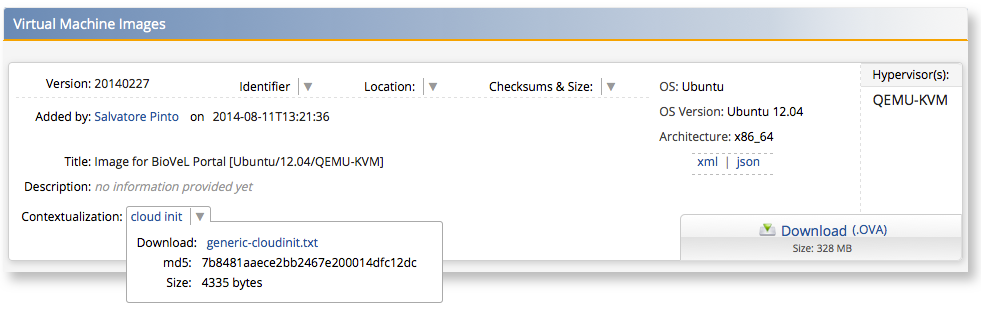
\includegraphics[width=\textwidth]{images/appdb_context}

  \end{block}
\end{frame}


\part{preparing-images}

%%%%%%%%%%%%%%%%%%%%%%%%%%%%%%%%%%%%%%%%%%%%%%%%%%%%%%%%%%%%%%%%%%%%%%%%%%%
\begin{frame}
  \frametitle{Windows}
  %\framesubtitle{FYI}

  \begin{block}{Windows can also be contextualizated!}
  \begin{itemize}
    \item cloud-init is linux-only, but
    \item cloudbase-init can help!
    \item Features:
    \begin{itemize}
        \item setting hostname 
        \item user creation
        \item group membership
        \item static networking
        \item SSH user's public keys
        \item user\_data custom scripts running in various shells (CMD.exe / Powershell / bash)
    \end{itemize}
  \end{itemize}
  \end{block}
\end{frame}


%%%%%%%%%%%%%%%%%%%%%%%%%%%%%%%%%%%%%%%%%%%%%%%%%%%%%%%%%%%%%%%%%%%%%%%%%%%

\begin{frame}[fragile]
  \frametitle{Windows}
  \framesubtitle{using cloudbase-init}
    
  \begin{block}{Installation}
    \begin{itemize}
        \item Installer available at \url{https://github.com/stackforge/cloudbase-init\#binaries}
        \item Installer can also execute sysprep if needed.
    \end{itemize}
  \end{block}

  \begin{block}{Contextualization}
    \begin{itemize}
        \item user-data can only be a script 
        \item but cloudbase-init will use all the meta-data 
    \end{itemize}
  \end{block}

\end{frame}

%%%%%%%%%%%%%%%%%%%%%%%%%%%%%%%%%%%%%%%%%%%%%%%%%%%%%%%%%%%%%%%%%%%%%%%%%%%

\part{Q \& A}

%%%%%%%%%%%%%%%%%%%%%%%%%%%%%%%%%%%%%%%%%%%%%%%%%%%%%%%%%%%%%%%%%%%%%%%%%%%

\begin{frame}
  \frametitle{Useful pointers}
  \framesubtitle{FedCloud \& Contextualization}

  \Fontsmaller

  \begin{block}{FedCloud}
  \begin{itemize}
    \item Wiki site -- \url{http://go.egi.eu/fedcloud}
    \item User support -- \url{https://wiki.egi.eu/wiki/Federated\_Cloud\_user\_support}
    \item User support e-mail -- \url{support@egi.eu}
    \item Cloud Marketplace -- \url{https://appdb.egi.eu/browse/cloud}
  \end{itemize}
  \end{block}

  \begin{block}{Contextualization}
  \begin{itemize}
    \item contextualization @ FedCloud -- \url{https://wiki.egi.eu/wiki/Fedcloud-tf:WorkGroups:Contextualisation}
    \item cloud-init -- \url{http://cloudinit.readthedocs.org/}
    \item cloudbase-init -- \url{https://github.com/stackforge/cloudbase-init}
  \end{itemize}
  \end{block}
\end{frame}

%%%%%%%%%%%%%%%%%%%%%%%%%%%%%%%%%%%%%%%%%%%%%%%%%%%%%%%%%%%%%%%%%%%%%%%%%%%

\begin{frame}
  \frametitle{Q \& A}
  \framesubtitle{}

  \begin{center}
    {\Huge ?}
  \end{center}
\end{frame}
 

\end{document}
